\documentclass[12pt,a4paper,fleqn,liststotocnumbered,bibtotocnumbered]{scrartcl}
\usepackage{htl}
\usepackage{tikz}
\usepackage{color, colortbl}
\usepackage{xcolor}
\usepackage{pdfpages}
\usepackage{mathtools}
\usepackage{amsmath}
\usepackage{upgreek}
\usepackage{float}
\usepackage{hyperref}
\usepackage{pgfplots}
\usepackage{listings}
\usepackage{matlab-prettifier}
\usetikzlibrary{arrows.meta}
\usepackage[nameinlink,capitalize]{cleveref}

\pgfplotsset{
    tick label style={/pgf/number format/fixed}
}


\Jahrgang{5BHET\,/\,2020/21}
\Titel{Feherbericht Master SPIN 220 PRO OPTO}
\Schueler{Stefan Deimel}

\sloppy
\definecolor{lightgray}{gray}{0.5}
\setlength{\parindent}{0pt}

\aboverulesep=0pt
\belowrulesep=0pt
\setlength{\parindent}{0pt}

\begin{document}
Der Motorregler ist bei niedriger Drehzahl (ca. 30\% - Gas) in Flammen aufgegangen. Die zuletzt empfangen Temperatur des Reglers waren etwa 20°C, die Spannung 58,5 V.
\\\\
Unser elektronsicher Aufbau:\\
Der Regler MASTER SPIN 220 PRO OPTO wird von 2 in Serie geschalteten 7S LiPo-Akkus (also insgesamt 14S) versorgt. Die Akkus sind 7500mAh-LiPos von Hacker (TopFuel LiPo 35C Power-X 7500mAh 7S MTAG). Der Motor ist ebenfalls von Hacker hergestellt (A200-6, siehe Rechnung).\\
Schaltplan:\\
{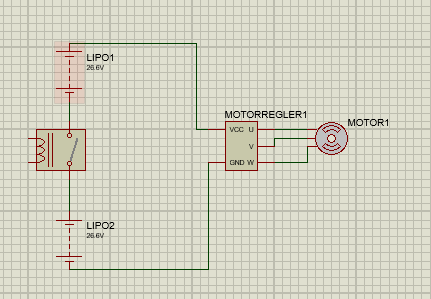
\includegraphics[width=.7\textwidth]{2021-02-22-21-04-18.png}}\\
Das Relay ist zum Ein- und Ausschalten der gesamten Elektronik.\\
\\
Wir verwenden den Motor mit 2x XOAR 3-Blatt Propeller als Schwebe-Antrieb für unser selbst gebautes Luftkissenboot.\\
\\
Wir bitten um Umtausch des Reglers auf Garantie.\\
Bei weiteren Fragen stehen wir gerne zur Verfügung.\\
\\
Wäre sehr nett wenn das Problem schnell gelöst werden könnte, da wir am 2. April die Diplomarbeit Abgeben müssen.\\
\\
Mit freundlichen Grüßen,\\
\\
Stefan Deimel (mailto: stefan.deimel@htlstp.at, Tel: +43 676 3939588),\\
Philipp Eilmsteiner,\\
Julia Stöger\\
\\
www.htlstp.ac.at\\
HTBLuVA St. Pölten\\
Waldstraße 3\\
3100 St. Pölten\\
AUSTRIA

\end{document}
